% Correcting the title chapter page
\fancypagestyle{plain}{%
    \fancyhf{}
    \fancyhead[RO,LE]{\bfseries \thepage}
    \fancyhead[CO]{\rightmark}
    \fancyhead[CE]{\leftmark}
    \renewcommand{\headrulewidth}{0.4pt}}

\chapter{Lieve grupe}
\label{ch:lie}

\section{Kontinuirane grupe}


- \emph{Konačne grupe} imaju binarnu operaciju (tablicu množenja)
koja zadovoljava četiri aksioma.

- elementima pridružujemo operatore $\to$ REPs i IREPS $\to$ moćni teoremi

- dokazi teorema o REPs su zasnovani na svojstvu konačnosti grupe

- Što ćemo s beskonačnim grupama (rotacija, translacija, Lorentzove transf.)?

Pristup:

- elementima konačne grupe možemo pridružiti konačan skup točaka u nekom
 prostoru $\to$ \emph{grupni prostor}

\centerline{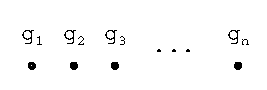
\includegraphics[scale=1.0]{pics/grupni_prostor.eps}}

- za \emph{kontinuirane beskonačne grupe} grupni prostor je tzv.
 \emph{mnogostrukost} tj. prostor lokalno sličan $\mathbb{R}^n$.

\secret{-Stroga def.: n-dim mnogostrukost je Husdorffov topološki
prostor u kojem je okolina svake točke homeomorfna $\mathbb{R}^n$.
(pravac, sfera, M\"{o}bius, dvostruki stožac nije, ...). Ideja je
generalizirati uobičajene plohe, ali bez uklapanja (embeddinga).}

- Npr. grupa rotacija oko neke osi $G=\{R(\theta) | \theta\in[0,2\pi)\}$
  ima kao grupnu mnogostrukost kružnicu (lokalno slična $\mathbb{R}^1$)

\centerline{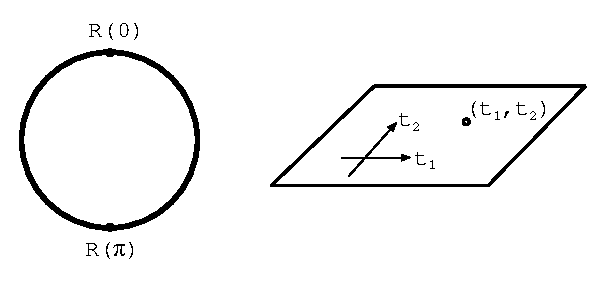
\includegraphics[scale=1.0]{pics/mnogostrukost.eps}}

- Npr. grupa translacija u ravnini: $\vec{x}\to\vec{x}+\vec{t}$,
  $\vec{t}=(t_1, t_2)$, $t_1, t_2 \in (-\infty, \infty)$ ima kao
 grupnu mnogostrukost ravninu = $\mathbb{R}^2$

- Elemente grupe označavamo s $n$ realnih brojeva (tzv. \emph{parametara}) 
  $(a_1, a_2, \ldots, a_n)$ koji određuju odgovarajuću točku na 
  grupnoj mnogostrukosti, te govorimo o \emph{$n$-parametarskoj grupi}.

- element grupe: $g(a_1, a_2, \ldots, a_n)\equiv g(a)$ (Npr. $R(\theta)$)

- Aksiomi grupe:

1) Zatvorenost: $g(c)=g(a)g(b) \in G$

    umjesto tablice množenja imamo funkciju $\phi: G\times G \to G \quad 
      c=\phi(a,b)$

2) Asocijativnost $g(a)[g(b)g(c)]=[g(a)g(b)]g(c)$ 
    $\imp \phi(a, \phi(b,c))=\phi(\phi(a,b),c) $

3) Identiteta: $\exists a^0 \td g(a^0)g(a)=g(a)g(a^0)=g(a)\quad \forall a$

    - reparametrizacijom mnogostrukosti možemo izabrati $a^0=(0, 0, \ldots, 0)
     \equiv 0$, $g(0)=e$ $\imp \phi(0,a)=\phi(a,0)=a$

4) Inverz: $\forall a\quad \exists \bar{a} \td g(a)g(\bar{a})=
        g(\bar{a})g(a)=g(0)=e$

    - $g(\bar{a})=g(a)^{-1}$

    - $\bar{a}=\psi(a) \quad \psi:G\to G$


Zasad nismo zatražili nikakvu povezanost između grupnih i topoloških
svojstava grupe. 


\begin{definicija}[Lieva grupa]
  Lieva grupa je kontinuirana grupa za koju su funkcije kompozicije
($\phi$) i inverza($\psi$) analitičke. (Često se još zahtijeva i
povezanost s jedinicom.)
\end{definicija}


Zahtjev da su te funkcije analitičke (te da je mnogostrukost
analitička) daje Lievim grupama mnoštvo važnih svojstava.

\secret{Strogo uzevši, analitičnost funkcije $\phi$ nije nužna tj. dovoljna
je kontinuiranost. (Ta činjenica je sadržaj rješenja 5. Hilbertovog
problema.)}

\centerline{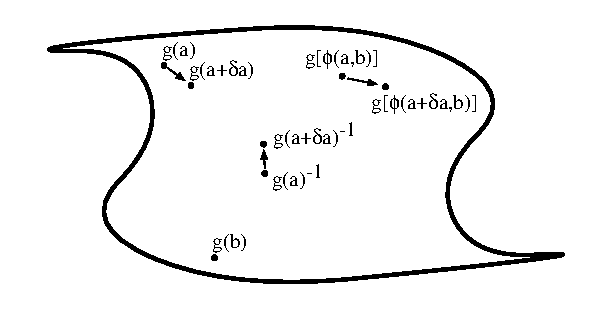
\includegraphics[scale=1.0]{pics/lieva_mnogostrukost.eps}}

Kontinuiranost grupe (preciznije, analitičnost mnogostrukosti) se ogleda
u činjenici da je element $g(a)$ ``blizu'' elementa $g(a+\delta a)$ dok
analitičnost funkcije kompozicije znači da je $\phi(a+\delta a, b)$
''blizu'' $\phi(a,b)$ tj. te su vrijednosti povezane Taylorovim redom.

Tako Lieve grupe spajaju ideje iz algebre i geometrije.

\section{Lieve algebre}
\label{sec:lievealgebre}

Neka su matrice $M(a)\equiv M(a_1, a_2, \ldots, a_n)$ elementi $n$-parametarske
Lieve grupe.
 
Za infinitezimalno male parametre $a_i \to \epsilon_i \ll 1$, zahvaljujući
analitičnosti možemo razviti oko $a_i = 0$:
\secret{(Cf. Cornwell Eq. (3.3))}
\begin{displaymath}
   M(\epsilon)=M(0)+ \sum_{i=i}^{n}\epsilon_i \frac{\partial M(a_1, \ldots, a_n)}
 {\partial a_i}\Bigg|_{a_1=\ldots =a_n=0} + 0(\epsilon^2)
\end{displaymath}


\begin{displaymath}
 \frac{\partial M(a_1, \ldots, a_n)}
 {\partial a_i}\Bigg|_{a_1=\ldots =a_n=0} = \textrm{const}(a_1, \ldots)
 \equiv  X_i  \quad i=1, \ldots, n \qquad \textrm{ - generatori grupe}
\end{displaymath}

- generatora ima koliko i parametara

\begin{displaymath}
  M(\epsilon_i)=\Eins + \epsilon_i X_i \qquad \textrm{ -
  infinitezimalne transformacije}
\end{displaymath}

- Želimo pokazati kako je struktura i REPs čitave grupe skoro sasvim
određena generatorima grupe tj. infinitezimalnom okolinom jediničnog 
elementa (ne gubimo ništa ograničavajući se na generatore, a njih
je lakše proučavati).

- Ne stignemo sve dokazati već ćemo većinu rezultata samo ilustrirati
  na primjeru grupe SO(3)


- rotacije oko $z$-osi --- jednoparametarska podgrupa od SO(3):

\begin{displaymath}
\left\{ R_3 (\phi) = \left( 
\begin{array}{ccc}
\cos\phi & -\sin\phi & 0 \\
\sin\phi & \cos\phi & 0 \\
0 & 0 & 1 
\end{array}
\right) \td \phi \in [0, 2\pi) \right\} \subset \textrm{SO(3)}
\end{displaymath}

\begin{displaymath}
X_3 = \frac{\partial R_3 (\phi)}{\partial \phi}\Bigg|_{\phi=0}=
\left( \begin{array}{ccc}
-\sin\phi & -\cos\phi & 0 \\
\cos\phi & -\sin\phi & 0 \\
0 & 0 & 1 
\end{array} \right)\Bigg|_{\phi=0} =
\left( \begin{array}{ccc}
0 & -1 & 0 \\
1 & 0 & 0 \\
0 & 0 & 0 
\end{array} \right)
\end{displaymath}

- infintezimalna rotacija: $R_3 (\epsilon) = 1 + \epsilon X_3$

- Kompozicija $N$ infinitezimalnih rotacija:

\begin{displaymath}
[R_3(\epsilon)]^{N} = (1+\epsilon X_3)^N = \left(1+\frac{(N\epsilon)X_3}
 {N}\right)^N \stackrel{\longrightarrow}{_{N\to\infty, (N\epsilon)\to\phi}}
 e^{\phi X_3}
\end{displaymath}

\begin{displaymath}
\exp\Bigg\{ 
\phi  \left( \begin{array}{ccc}
0 & -1 & 0 \\
1 & 0 & 0 \\
0 & 0 & 0 
\end{array} \right)\Bigg\} =\left( 
\begin{array}{ccc}
\cos\phi & -\sin\phi & 0 \\
\sin\phi & \cos\phi & 0 \\
0 & 0 & 1 
\end{array}
\right)
\end{displaymath}

(Ovo smo eksplicitno eksponencirali na vježbama.)

$\to$ konačni (dakle svaki) element jednoparametarske podgrupe
od SO(3) dobivamo eksponencijacijom generatora 

- Nadalje, u skladu s Eulerovim teoremom iz mehanike\footnote{Svaki pomak krutog
tijela kod kojeg jedna točka ostaje nepomična je ekvivalentan \emph{jednoj}
rotaciji oko fiksne osi koja prolazi kroz tu točku.} svaka SO(3) rotacija 
pripada nekoj jednoparametarskoj podgrupi
 (podgrupu čine sve rotacije oko te iste osi), što znači da se
 svi elementi SO(3) mogu se dobiti eksponencijacijom generatora

-$X_1$, $X_2$, $X_3$=? \quad\textrm{ovise o parametrizaciji grupnog prostora}

- Mogli bismo konstruirati opći element SO(3) grupe kao kompoziciju tri
 Eulerove rotacije i onda deriviranjem po 3 Eulerova kuta dobiti tri
 generatora grupe. No, ima i lakši put koji će olakšati traženje 
 generatora drugih Lievih grupa koje se pojavljuju u fizici. 
 (Usput, pristup preko Eulerovih
 rotacija je problematičan jer su one singularne oko jedinice.):

SO(3) je grupa svih 3$\times$3 matrica $R$ sa svojstvima  
  $RR^{T}=1$ i $\det R=1$

- $R(\epsilon)=1+\epsilon X \imp RR^{T}=(1+\epsilon X)(1+\epsilon 
   X^{T}) = 1+\epsilon (X+X^{T})+0(\epsilon^2) = 1$

$\imp X^T=-X \imp X$ je antisimetrična 3$\times$3 matrica (čime je uvjet
$\det R=1$ automatski ispunjen - vidi 
   $\det R = e^{\theta\textrm{\scriptsize Tr} X}$ sa vježbi

- skup $\calA$ svih antisimetričnih 3$\times$3 matrica generira grupu SO(3)

- No, taj skup je i vektorski prostor: $X_1,X_2\in\calA\imp
    (\alpha X_1 + \beta X_2)\in\calA \quad \forall \alpha, \beta\in\mathbb{R}$

- dim($\calA$)=3

- Uobičajenu bazu čine generatori jednoparametarskih podgrupa rotacija oko
  $x$, $y$ i $z$ osi

\begin{equation}
X_1=\left(
\begin{array}{ccc}
0 & 0 & 0 \\ 
0 & 0 &-1 \\
0 & 1 & 0
\end{array} \right) \quad
X_2=\left(
\begin{array}{ccc}
0 & 0 & 1 \\ 
0 & 0 & 0 \\
-1& 0 & 0
\end{array} \right) \quad
X_3=\left(
\begin{array}{ccc}
0 & -1 & 0 \\ 
1& 0 & 0 \\
0 & 0 & 0
\end{array} \right) \quad
\label{eq:SO3generators}
\end{equation}

- $e^{\phi \vec{X}\cdot\unitn}$ je onda općeniti element grupe SO(3)

- Vektorski prostor je bogatija struktura od grupe što generatore
 čini zanimljivijim nego same elemente grupe.

- No postoji i dodatno važno svojstvo: Neka su $X,Y\in\calA$.

$[X,Y]^T = (XY-YX)^T = Y^T X^T - X^T Y^T = YX-XY = -[X,Y] \imp [X,Y]\in\calA$

- Dakle, $\calA$ je zatvoren ne samo obzirom na linearne kombinacije već
   i obzirom na komutatore svojih elemenata $\to$ \emph{Lieva algebra}

\begin{definicija}[Lieva algebra]
Lieva algebra $\calA$ je vektorski prostor na kojem je definiran 
Liev produkt dvaju elemenata $[X,Y]$ (ne mora biti komutator) sa svojstvima

1) zatvorenost: $[X,Y]\in\calA \quad \forall X,Y\in\calA$

2) distributivnost: $[\alpha X + \beta Y, Z]=\alpha[X,Z]+\beta[Y,Z]$
$\quad \alpha,\beta \in \mathbb{R} (\mathbb{C} \to \textrm{kompleksna L.a.})$

3) antisimetrija: $[X,Y]=-[Y,X]$

4) Jacobijev identitet: $[X, [Y, Z]]+[Y, [Z, X]]+[Z, [X, Y]]=0$
\end{definicija}

\secret{Za \emph{algebru} generički, vidi Cvitanović p. 17.}

Za vektorske prostore matrica, gdje je Liev produkt definiran kao
komutator $[X,Y]=XY-YX$, svojstva 2--4 su automatski ispunjena.

\textbf{Teorem (Ado)}: Svaka konačno-dimenzionalna apstraktna Lieva algebra je izomorfna nekoj
 Lievoj algebri konačno-dimenzionalnih matrica s komutatorom kao Lievim produktom. \emph{(Bez
dokaza.)}

Dakle, ograničavajući se na Lieve grupe \emph{matrica} ne gubimo mnogo
na općenitosti jer sve Lieve algebre koje ćemo sresti u ovoj knjizi su
konačno-dimenzionalne\footnote{Istina, u fizici nekad nalazimo i primjenu beskonačno-dimenzionalnih
algebri za koje teorem ne vrijedi. Jedan primjer je tzv. Virasorova algebra važna
u teoriji superstruna.}.

- Lieve algebre ponekad označavamo isto kao i Lieve grupe, ali malim slovima:
  $X_1$, $X_2$ i $X_3$ su baza Lieve algebre so(3).

$X_i, i=1,2,\ldots, \textrm{dim}(\calA)$ - baza vektorskog prostora 
  $\imp [X_i, X_j]\in\calA$

$\imp [X_i, X_j]=C_{ij}^{k}X_k  \quad i,j=1,2,\ldots, \textrm{dim}(\calA)$

$C_{ij}^{k}$ - \emph{strukturne konstante}

\begin{primjer}[strukturne konstante od SO(3)]
$[X_i,X_j]=0$ za $i=j$ 

$[X_1,X_2] = X_3$

\secret{Provjeri eksplicitno... Slično,}

$[X_2, X_3]=X_1$ 

$[X_3,X_1]=X_2$

$C_{ij}^{k}=0$ ako su bilo koja dva indeksa ista

$C_{12}^3=C_{23}^{1}=C_{31}^{2}=1$

$C_{21}^3=C_{32}^{1}=C_{13}^{2}=-1$

\end{primjer}

\rule{3cm}{0.5pt}

\textbf{Digresija:} \emph{Levi-Civita pseudotenzor}

Levi-Civita ili totalno antisimetrični pseudotenzor trećeg reda definiran
je svojim komponentama $\epsilon_{ijk}$ tako da je
\begin{displaymath}
\epsilon_{ijk}=
\begin{cases}
1& \text{ako je $(i,j,k)$ parna permutacija od $(1,2,3)$}, \\
-1& \text{ako je $(i,j,k)$ je neparna permutacija od $(1,2,3)$}, \\
0& \text{inače, tj. ako su dva ili sva tri indeksa ista}.
\end{cases} 
\end{displaymath}

Npr. $\epsilon_{231}=1$, $\epsilon_{213}=-1$, $\epsilon_{221}=0$, itd.
Pomoću Levi-Civita tenzora, komutacijske relacije algebre SO(3) pišemo
\begin{displaymath}
 [X_i, X_j]=\epsilon_{ijk} X_k  
\end{displaymath}

Levi-Civita tenzor je od velike pomoći u računima (vidi vježbe).
Za definiciju pojma ``tenzor'' vidi poglavlje \ref{ch:klasicna}, no tenzorsko
svojstvo Levi-Civita tenzora će nam u praksi biti nebitno.

\rule{3cm}{0.5pt}

Lieva algebra $\calA'$ je \emph{homomorfna} Lievoj algebri $\calA$ ako postoji 
operator $S:\calA\to\calA'$ tako da je
\begin{displaymath}
       [S(X), S(Y)]=S([X,Y]) \quad \forall X, Y \in\calA
\end{displaymath}
Ako je $S$ još i bijekcija $\calA$ i $\calA'$ su \emph{izomorfne}.

\begin{primjer}[Lieva algebra grupe SU(2)]
 čine je sve antihermitske\footnote{$A$ je antihermitska ako je $A^\dagger=-A$} 
2$\times$2 matrice s tragom nula Baza je 
\[
     \{ -i\frac{\sigma_1}{2},  -i\frac{\sigma_2}{2},  -i\frac{\sigma_3}{2} \}
\]
gdje su $\sigma_{1,2,3}$ tri Paulijeve matrice:
\begin{equation}
\sigma_1=\left( \begin{array}{cc} 0 &  1 \\ 1 & 0 \end{array} \right)
\quad
\sigma_2=\left( \begin{array}{cc} 0 & -i \\ i & 0 \end{array} \right)
\quad
\sigma_3=\left( \begin{array}{cc} 1 &  0 \\ 0 &-1 \end{array} \right)
\label{eq:PaulijeveMatrice}
\end{equation}
Ova tri generatora zadovoljavaju iste komutacijske relacije kao i matrice
SO(3) algebre
\begin{displaymath}
 \left[ -i\frac{\sigma_1}{2}, -i\frac{\sigma_2}{2} \right] =
 -i\frac{\sigma_3}{2} \qquad \text{itd.}
\end{displaymath}
pa je $X_i \to -i \sigma_i/2$ ($i=1,2,3$) izomorfizam.
so(3)=su(2).

(D.Z. Uvjerite se da je su(2) \emph{realna} Lieva algebra, dakle algebra
nad poljem $\mathbb{R}$, premda su elementi matrica općenito kompleksni.)
\end{primjer}

Pojmovi REP i IRREP za Lieve grupe imaju isto značenje kao i za
konačne grupe (dakle to je grupa operatora na nekom vektorskom prostoru
homomorfna grupi). Lievim algebrama možemo također pridijeliti
njihove vlastite reprezentacije.

Zapravo, cijela dosadašnja diskusija je i bila o 
\emph{reprezentacijama} grupe/algebre  SO(3) na 3D euklidskom 
vektorskom prostoru.

\begin{definicija}[Casimirov operator]
Ako je skup $\{L_i, i=1,2, ... \}$ baza Lieve algebre onda se polinom
u $L_i$ koji komutira sa svim elemetnima te algebre naziva 
\emph{Casimirov operator}.
\end{definicija}

- Posebno su zanimljivi kvadratični Casimirovi operatori.

\begin{primjer}
$X_{1}^2 + X_{2}^2 + X_{3}^2 = -2 \Eins $

Schurova lema (vrijedi i za Lieve grupe) traži da Casimirov operator 
bude proporcionalan jediničnom što je onda zgodno za označavanje IRREPSa.
\end{primjer}

\section{Veza Lievih grupa i Lievih algebri$^*$}

U slučaju grupe SO(3) smo, zahvaljujući Eulerovom teoremu, vidjeli da
\emph{svaki} element grupe možemo prikazati kao eksponencijal jednog
elementa iz Lieve algebre so(3).

Pitanje je da li se ovo poopćava na proizvoljnu Lievu grupu.

Odgovor je: Skoro, ali ne sasvim. Vrijedi \emph{(bez dokaza)}:

1) Svakoj Lievoj grupi jednoznačno pripada neka Lieva algebra. Svaki 
  se element iz neke male (ne nužno infinitezimalne!) okoline 
  jediničnog elementa grupe može
  prikazati u obliku $e^{t X}$ gdje je $t$ realni parametar, a $X$ element
  te Lieve algebre.

2) Ako je Lieva grupa kompaktna, onda se "mala okolina" proširuje na
   čitavu komponentu povezanosti jedinice.

\emph{kompaktna} = parametri variraju po zatvorenim intervalima\\
   Npr. SO(3) je kompaktna, a grupa translacija nije. SO(n) i SU(n) su
 kompaktne, a najzanimljivije su nam za QM.

\emph{komponenta povezanosti jedinice} = svi elementi grupe koji se
kontinuiranom linijom u grupnoj mnogostrukosti mogu povezati s
jediničnim elementom\\
 Npr. sve obične rotacije su u komponenti povezanosti
jedinice, dok refleksije nisu.

\secret{Ako nije kompaktna, svejedno se elementi iz komponente
povezanosti jedinice mogu prikazati kao konačan umnožak eksponencijala
$e^{t_1 X_1} e^{t_2 X_2}\cdots e^{t_n X_n}$}

Što se \emph{strukture} grupe tiče tj. njene ``tablice množenja'', važnu
ulogu ima formula
\begin{equation}
\begin{split}
  e^A e^B &= \exp\Bigg\{A+B+\frac{1}{2}[A,B]+\frac{1}{12}\Big(\big[A,[A,B]\big]+
 \big[B,[B,A]\big]\Big)+\cdots \Bigg\} \\
          &= f(A,B,[A,B]) \qquad \text{\emph{(Baker-Campbell-Hausdorff ili BCH teorem)}}
\end{split}
\end{equation}

Ovaj red konvergira u određenoj okolini jedinice (ne nužno infinitezimalnoj!)
u kojoj onda algebra \emph{potpuno} određuje grupu.

To je dubok rezultat i puni dokaz BCH teorema obično zahtijeva napredne matematičke
pojmove. Relativno pristupačan algebarski dokaz može se pronaći u knjizi
Stilvell, \emph{Naive Lie Theory}.

(D.Z. Provjerite BCH formulu do gore navedenog reda.)

Pitanje: Da li istoj Lievoj algebri mogu pripadati različite Lieve grupe?

Primjer grupa SO(3) i SU(2) koje imaju istu algebru sugerira da je to moguće. 
(Ako SO(3) i SU(2) nisu izomorfne grupe, a vidjet ćemo na vježbama da nisu.)

Da bismo precizno opisali vezu između Lievih grupa s istom algebrom, treba
nam pojam \emph{povezanosti}

\begin{definicija}[Povezanost]
  Neka je G povezana grupa (ako nije, možemo promatrati samo komponentu
povezanosti jedinice). Promotrimo skup svih zatvorenih krivulja u grupnoj 
mnogostrukosti. Podijelimo skup  na klase ekvivalencije koje čine 
krivulje koje se mogu \emph{kontinuirano} deformirati jedna u drugu.
Broj takvih klasa zovemo \emph{povezanost} grupe G. Ako postoji samo
jedna klasa kažemo da je grupa \emph{jednostavno} ili \emph{jednostruko}
povezana.
\end{definicija}

\begin{primjer}[U(1)]
$u u^\dagger = u u^* = 1 \imp |u|=1 \imp u=e^{i\phi} \imp$ grupna
mnogostrukost je kružnica.
(Usput, U(1)=SO(2). D.Z.: Pronađite izomorfizam.)
Za zatvorene krivulje promjena kuta $\phi$ duž krivulje je $2n\pi$,
$n=0,\pm 1, \pm 2, \ldots$. Krivulje s različitim $n$ pripadaju
različitim klasama povezanosti $\to$ U(1) je beskonačno povezan.

\centerline{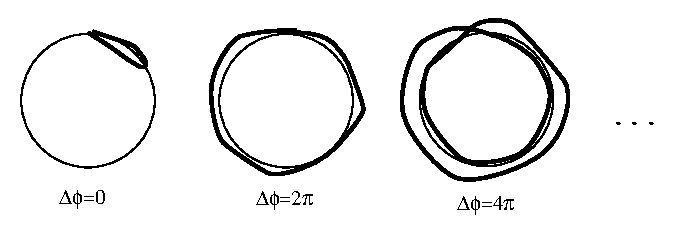
\includegraphics[scale=1.0]{pics/homotopija.eps}}

Digresija: Moguće je na prirodan način definirati zbrajanje (klasa) krivulja 
obzirom na koje skup ovih klasa čini grupu --- tzv. \emph{fundamentalnu
grupu} ili \emph{prvu grupu homotopija} $\pi_1$. Ovdje $\pi_1=(\mathbb{Z}, +)$.

\end{primjer}

\begin{primjer}[SO(3)]
Kako izgleda parametarski prostor od SO(3)? Element od SO(3) je definiran
smjerom osi rotacije i iznosom kuta rotacije pa se grupna mnogostrukost
može prikazati kao puna lopta promjera $\pi$ s identificiranim nasuprotnim
točkama površine sfere:

\centerline{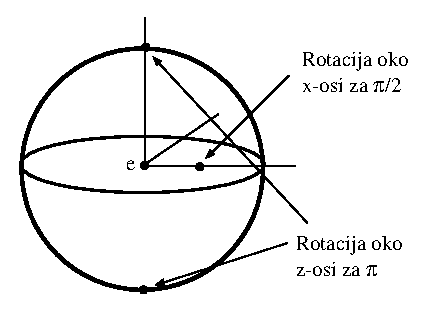
\includegraphics[scale=0.8]{pics/so3mnogostrukost.eps}}

Svaka rotacija je u pozitivnom smjeru. Rotacije za kuteve $(\pi, 2\pi)$ se dobiju
suprotno usmjerenim osima. Identifikacija nasuprotnih točaka je posljedica
činjenice da je su rotacije za $\pi$ oko suprotno usmjerenih osi
identične.

\centerline{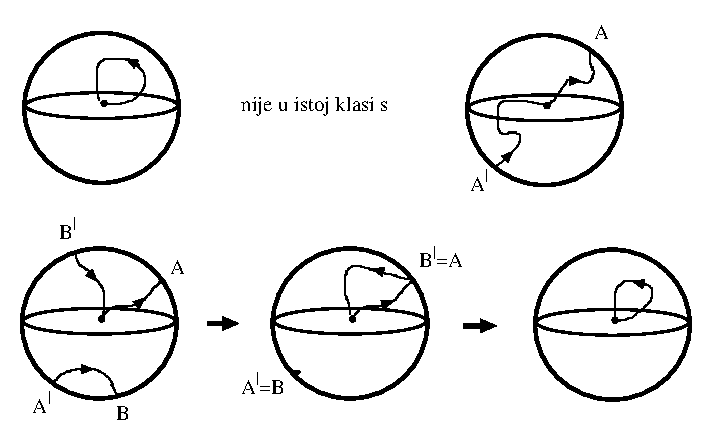
\includegraphics[scale=0.8]{pics/dvostruka_povezanost_so3.eps}}

Dakle, SO(3) je dvostruko povezana.
\end{primjer}

\begin{primjer}[SU(2)]
Grupna mnogostrukost od SU(2) je 3-sfera tj. generalizacija uobičajene
sfere (2-sfere) na četverodimenzionalni prostor. (Vidi vježbe za ovo.)
Može se pokazati da je svaka $n$-sfera s $n>1$ jednostavno povezana.
\secret{Hamermesh, p.320, stereografskom projekcijom se pokazuje
da je $S^n$ bez jedne točke homeomorfan $\mathbb{R}^n$. \emph{``You
cannot lasso a sphere''}}
\end{primjer}

Ako postoji homomorfizam s povezane Lieve grupe G na povezanu Lievu
grupu H s \emph{diskretnom} jezgrom K onda kažemo da grupa G 
\emph{pokriva} grupu H onoliko puta koliko elemenata ima K.
(Prisjetite se teorema \ref{th:izomorfizam} o izomorfizmu.)
Također, Lieve algebre tih grupa su izomorfne.

\begin{primjer}[SO(3) i SU(2)]
SO(3) i SU(2) su homomorfne. Sam homomorfizam ćemo konstruirati na 
vježbama gdje ćemo vidjeti da je on 2-1 s SU(2) na SO(3) tj. jezgra
K ima dva elementa. Dakle SU(2) pokriva SO(3) dva puta.
\end{primjer}

\begin{teorem}
Među grupama koje pokrivaju povezanu Lievu grupu G, postoji jedinstvena
grupa koja je jednostavno povezana --- \emph{univerzalna grupa pokrivanja}.
Broj pokrivanja jednak je povezanosti od G. \emph{(Bez dokaza)}
\end{teorem}

Npr. SU(2) je univerzalna grupa pokrivanja za SO(3). Prema
teoremu o izomorfizmu  SU(2)/$\{1,-1\}$=SO(3).\\[1ex]

\centerline{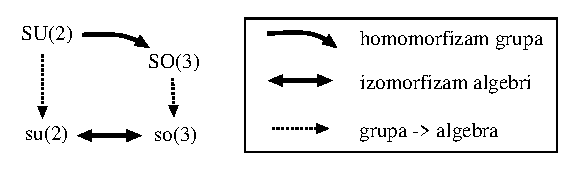
\includegraphics[scale=1.0]{pics/so3pokrivanje.eps}}

Općenita situacija je\\[1ex]

\centerline{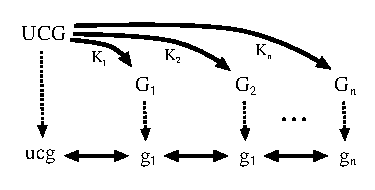
\includegraphics[scale=1.0]{pics/ucg.eps}}

gdje je UCG/$K_i$=G$_i$. Pronalaženjem svih diskretnih invarijantnih
podgrupa od UCG možemo naći sve grupe njoj lokalno izomorfne.

\rule{3cm}{0.5pt}

   Bliska povezanost grupe SU(2) s grupom rotacija SO(3) sugerira da
bi ona mogla imati i fizikalni značaj. Trikovi s pojasom\footnote{Zakretanjem
originalno vodoravnog pojasa držanjem za kopču kreiramo jednu zatvorenu putanju
u grupi SO(3): kut i smjer su dani zakrenutošću pojedinog intervala
pojasa i njegovom udaljenošću od ravnog vodoravnog položaja. 
Kopča mora biti vodoravna kao i zavezani drugi kraj pojasa da bi
oba kraja odgovarala identiteti. Jednom zakrenuti pojas nikakvim kontinuiranim
transformacijama (koje drže kopču vodoravnom) ne možemo izravnati pojas; dvaput
zakrenuti pojas možemo izravnati prebacivanjem remena preko kopče.}
 ili konobarevim
pladnjem pokazuju da rotacije za 360$^\circ$ zaista nisu uvijek u svakom pogledu
identične rotaciji za 0$^\circ$, dok one za 720$^\circ$ stupnjeva to jesu.
Također, Hamiltonova demonstracija da se komponiranje rotacija prirodnije
izvodi pomoću kvaterniona (skup kvaterniona je ekvivalentan SU(2) grupi) 
dodatno sugerira da ta grupa nije sasvim apstraktna.
  I stvarno, pokazuje se da se neki sustavi u prirodi (tzv. fermionski
sustavi) trasformiraju pri rotacijama kao reprezentacije SU(2) grupe
(vidi 6. poglavlje)
i to je i eksperimentalno potvrđeno npr. u eksperimentima s neutronskom
interferometrijom. \secret{(cf. Sakurai)}

\section{Primjeri Lievih grupa važnih za fiziku}

\begin{enumerate}
\item \textbf{Opća linearna grupa}

$GL(n, \mathbb{C})$ --- skup svih $n\times n$ regularnih ($\det M \neq 0$)
kompleksnih matrica

Kako je svaka matrica zadana s $n^2$ nezavisnih kompleksnih brojeva, ova
grupa ima $2 n^2$ realnih parametara. Uvjet regularnosti nije ograničenje
koje smanjuje broj parametara, jer je samo riječ o zahtjevu da determinanta,
koja je izraz koji uključuje tih $2 n^2$ parametara bude \emph{različita} od nule.

\begin{equation}
\det M = f(a_1, a_2 , \dots, a_{2n}) \neq 0
\end{equation}

Podgrupa ove grupe je grupa $GL(n, \mathbb{R})$ koja očito ima samo
$n^2$ parametara.

\item \textbf{Specijalna linearna grupa}

\begin{equation}
SL(n, \mathbb{C}) = \{ M\in GL(n,\mathbb{C}) \; | \; \det M = 1\}
\end{equation}

Ovdje je na svaku matricu postavljen dodatni uvjet
\begin{equation}
\det M = f(a_1, a_2 , \dots, a_{2n}) = 1 \;,
\label{eq:SL}
\end{equation}
koji predstavlja jednu kompleksnu, tj. dvije realne jednadžbe koje
se mogu iskoristiti za eliminaciju dvaju parametera. Tako ova grupa
ima $2 n^2 - 2$ parametra.

Podgrupa ove grupe je grupa $SL(n, \mathbb{R})$ koja ima 
$n^2 - 1$ parametar. (Jednadžba (\ref{eq:SL}) je sad samo jedna
realna jednadžba, a ne dvije.)

\item \textbf{Unitarna grupa}

\begin{equation}
U(n) = \{ M\in GL(n,\mathbb{C}) \; | \; M M^{\dagger} = 1\}
\end{equation}

Prebrojavanje nezavisnih parametara za ovu grupu može se izvesti
na više načina. Uvjet $M M^\dagger = 1$ se može napisati izraženo
preko komponenti matrica kao:
\begin{equation}
\sum_{j=1}^{n} M_{ij} M_{kj}^* = \delta_{ik}\;,
\label{eq:unitaritycondition}
\end{equation}
gdje je iskorišteno $M^{\dagger}_{jk} = M^{*}_{kj}$.
Jednadžba (\ref{eq:unitaritycondition}) predstavlja $n^2$ kompleksnih
jednadžbi ali sve one nisu nezavisne. Promotrimo prvo $n$ jednadžbi
određenih uvjetom $i=k$ (dakle gledamo dijagonalu te matrične jednadžbe):
\begin{equation}
 \sum_j M_{ij} M^{*}_{ij} = \sum_j |M_{ij}|^2 = 1
\label{eq:diagonalcondition}
\end{equation}
To je $n$ realnih jednadžbi koje se mogu upotrijebiti za eliminiranje
$n$ parametara. Dalje možemo gledati jednadžbe određene uvjetom
$i < k$ (dakle gledamo trokut iznad dijagonale matrične jednadžbe).
Te su jednadžbe kompleksne i ima ih $n(n-1)/2$ (broj elemenata u 
spomenutom trokutu). Sve ove jednadžbe su neovisne pa se mogu
iskoristiti za eliminranje $2 \cdot n(n-1)/2 = n(n-1)$ parametara.
Preostaju jednadžbe za $i >k$ (donji trokut matrice), ali kompleksnom
konjugacijom odgovarajućih jednadžbi
\begin{equation}
\sum_{j=1}^{n} M_{ij} M_{kj}^* = 0\;, \qquad i>k
\end{equation}
dobijemo
\begin{equation}
\sum_{j=1}^{n} M_{ij}^* M_{kj}  = \sum_{j=1}^{n} = M_{kj} M_{ij}^* = 0\;, \qquad i>k
\end{equation}
pa uz preimenovanje indeksa $i \leftrightarrow k$
\begin{equation}
\sum_{j=1}^{n} =  M_{ij} M_{kj}^* = 0\;, \qquad k>i
\end{equation}
vidimo da su ove jednadžbe ekvivalentne ovima iz gornjeg trokuta tj. nisu
nezavisne.
Znači sve skupa možemo eliminirati $n + n(n-1) = n^2$ parametara, pa ih
ostane $2n^2 - n^2 = n^2$ što je broj parametara unitarne grupe.
(Drugi način prebrojavanja je da se iskoristi da su retci matrice ortonormirani
vektori. Uvjet normalizacije daje $n$ realnih jednadžbi, a uvjet
ortonogonalnosti $\binom{n}{2}$ kompleksnih, gdje se treba uvjeriti
da odgovarajući zahtjevi na stupce nisu nezavisni od ovih na retke.)

Važno svojstvo unitarnih matrica je da, ukoliko ih interpretiramo kao
operatore nad kompleksnim vektorskim prostorima ($\vec{x} \to M\vec{x}$), 
one čuvaju skalarni produkt
\begin{align}
  (x, y)& = \sum_{i=1}^n x_{i}^* y_i  \longrightarrow
   \sum_{ijk} M^{*}_{ij}x^{*}_j M_{ik}y_{k} \nonumber \\
 & = \text{uvrštavanjem
(\ref{eq:unitaritycondition})} = \sum_{kj} \delta_{kj} x^{*}_j y_k = (x, y)
\label{eq:productinvariance}
\end{align}
Lako je pokazati (D.Z.) da se ovo može uzeti kao alternativna definicija
unitarne grupe tj. da se unitarne matrice mogu definirati kao one koje
čuvaju ovaj skalarni produkt, a onda je svojstvo $M^{\dagger} M = 1$, koje
smo ovdje uzeli kao definiciono, samo posljedica.

\item \textbf{Specijalna unitarna grupa}

\begin{equation}
SU(n) = \{ M\in U(n) \; | \; \det M  = 1\}
\end{equation}

Za prebrojavanje parametara treba prvo uočiti da je za sve unitarne
matrice determinanta ograničena na apsolutnu vrijednost 1. To slijedi
primjenom Binet-Cauchyjevog teorema na definiciju $M M^{\dagger} = 1$
što daje $|\det M|^2 = 1$ odnostno $\det M = e^{i \phi}$, 
$\phi\in [0, 2\pi)$.
Dodatni uvjet za specijalne unitarne matrice $\det M = 1$ je onda
samo jedna realna jednadžba $\phi = 0$ pa specijalna unitarna grupa
ima točno $n^2 - 1$ parametar.

\item \textbf{Ortogonalna grupa}

\begin{equation}
O(n, \mathbb{C}) = \{ M\in GL(n,\mathbb{C}) \; | \; M M^{\mathrm{T}} = 1\}
\end{equation}

Kod prebrojavanja uvjeta, jedina razlika obzirom na unitarne matrice
je da umjesto ($i=k$) jednadžbi (\ref{eq:diagonalcondition}) 
koje odgovaraju dijagonali matrične jednadžbe sada imamo
\begin{equation}
 \sum_j M_{ij} M_{ij} = \sum_j M_{ij}^2 = 1
\end{equation}
što su kompleksne jednadžbe pa možemo eliminirati sve skupa
$2n + n(n-1)$ parametara i ostaje ih samo $n(n-1)$.

U fizici se najčešće susrećemo s grupom ortogonalnih \emph{realnih} matrica
\begin{equation}
O(n) \equiv O(n, \mathbb{R}) = \{ M\in GL(n,\mathbb{R}) \; | \; M M^{\mathrm{T}} = 1\}
\end{equation}
koja ima $n(n-1)/2$ parametara. (Uvjerite se u to.) Ova grupa čuva
kvadratnu formu $\sum_i x_i y_i$ (skalarni produkt na realnom
vektorskom prostoru) što se može upotrijebiti kao alternativna definicija.

\item \textbf{Specijalna ortogonalna grupa}

\begin{equation}
SO(n, \mathbb{C}) = \{ M\in O(n, \mathbb{C}) \; | \; \det M  = 1\} \;,
\end{equation}
i odgovarajuća realna grupe $SO(n)$ imaju isti broj parametara kao
$O(n, \mathbb{C})$, odnosno $O(n)$. Naime, uvjet ortogonalnosti
$M M^{\mathrm{T}} = 1$ opet uz primjenu Binet-Cauchyjevog teorema vodi
na $(\det M)^2 = 1$, odnosno
na zaključak da ortogonalne matrice imaju determinantu $\det M = \pm 1$,
pa ograničenje na $\det M = 1$ ne smanjuje dimenziju parametarskog prostora.

\item \textbf{Pseudo-unitarna grupa}

Čine je $n\times n$ matrice
\begin{equation}
U(p, q) = \{ M\in GL(n,\mathbb{C}) \; | \; M^{\dagger} g M = g\} \;,
\end{equation}
gdje je $p+q=n$ i gdje je $g$ dijagonalna matrica oblika
\begin{equation}
  g = \mathrm{diag}(\underbrace{1, 1, \dots, 1}_{p \times},
\underbrace{-1, -1, \dots, -1}_{q \times}) \;.
\label{eq:metricg}
\end{equation}

Ova grupa ima isti broj parametara kao i $U(n)$, te
čuva kvadratnu formu oblika
\begin{equation}
 \sum_{i=1}^{p} x_{i}^* y_{i} - \sum_{i=p+1}^{p+q=n} x_{i}^* y_i 
\end{equation}
koja nije pozitivno definitna pa nije skalarni produkt u smislu
definicije \ref{def:skalarniprodukt}.


\item \textbf{Pseudo-ortogonalna grupa}

\begin{equation}
O(p, q) = \{ M\in GL(n,\mathbb{R}) \; | \; M^{\mathrm{T}} g M = g \} \;,
\end{equation}
gdje je $p+q=n$ i gdje je $g$ dijagonalna matrica iz (\ref{eq:metricg}).
Ove matrice čuvaju kvadratnu formu oblika
\begin{equation}
 \sum_{i=1}^{p} x_{i} y_{i} - \sum_{i=p+1}^{p+q=n} x_{i} y_i  \;.
\end{equation}
Najpoznatija grupa ove vrste je grupa Lorentzovih transformacija  $O(1,3)$
(vidi odjeljak \ref{sec:lorentz}).

Specijalnu pseudo-unitarnu grupu $SU(p,q)$ odnosno specijalnu pseudo-ortogonalnu
grupu $SO(p,q)$ dobivamo ako se u $U(p,q)$ odnosno $O(p, q)$
ograničimo na matrice s $\det M = 1$.

\end{enumerate}

\subsection{Topološka svojstva Lievih grupa$^*$}

\begin{itemize}
\item $GL(n, \mathbb{C})$ je očito nekompaktna (svi elementi matrica
slobodno poprimaju vrijednosti iz skupa $(-\infty, \infty)$ i povezana
(kontinuiranim promjenama elemenata svaku matricu možemo pretvoriti u
jediničnu).

\item $GL(n, \mathbb{R})$ je isto nekompaktna. Što se tiče povezanosti,
treba uočiti da je determinanta kontinuirana funkcija elemenata matrice
čija je vrijednost realni broj iz $(-\infty, 0) \cup (0, \infty)$
(zahtjev postojanja inverza isključuje nulu). To znači da kontinuiranim
promjenama parametara ne možemo matrice s negativnim determinantama
pretvoriti u jediničnu i ova grupa ima dvije odvojene komponente povezanosti.

\item Na sličan način možemo zaključiti da grupa $O(n)$, gdje je
determinanta $\pm 1$, isto ima dvije komponenete povezanosti, s time
da je ova grupa kompaktna --- parametri su kutevi rotacija koji poprimaju
vrijednosti iz kompaktnih skupova poput $[0, 2\pi\equiv0)$.

\item $U(n)$ i $SU(n)$ su kompaktne povezane grupe, gdje je $SU(n)$ još i
jednostavno povezana.

\item $O(p, q)$ je nekompaktna grupa s četiri komponente povezanosti
što za konkretan primjer grupe $O(1,3)$ pokazujemo u odjeljku \ref{sec:lorentz}.

\end{itemize}

\subsection*{Zadaci za vježbe}

\begin{enumerate}[label=\arabic{chapter}.\arabic*.]

\item Primjeri eksponenciranja matrica.

\item \label{zad:LeviCivitaProperties} Pokažite da Levi-Civita tenzor ima slijedeća svojstva:
\begin{align*}
\tag{a}\epsilon_{ijk}\epsilon_{imn}&=\delta_{jm}\delta_{kn}-\delta_{jn}\delta_{km}\\
\tag{b}\epsilon_{ijk}\epsilon_{ijm}&=2\delta_{km} \\
\tag{c}\epsilon_{ijk}\epsilon_{ijk}&=6 \\
\tag{d}\epsilon_{ijk}a_j b_k &= (\vec{a}\times\vec{b})_i  \\
\tag{e}\frac{1}{3!}\epsilon_{lmn} \epsilon_{ijs} A_{li} A_{mj} A_{ns} &= \det A
\end{align*}

\item Uporabom svojstava Levi-Civita tenzora pokažite da je
za vektore $\vec{a}$, $\vec{b}$ i \vec{c}
\begin{displaymath}
    \vec{a}\times(\vec{b}\times\vec{c})=(\vec{a}\cdot\vec{c})\vec{b}
 -(\vec{a}\cdot\vec{b})\vec{c}
\end{displaymath}
\secret{Za slične stvari vidi Evett, Am. J. Phys \textbf{34} (1966) 503.}

\item Pokažite da Paulijeve matrice imaju slijedeća svojstva:
\begin{align*}
\tag{a} \sigma_{i}^2 &= 1 \\
\tag{b} \sigma_{i}^\dagger &= \sigma_i \\
\tag{c} \det \sigma_i &= -1 \\
\tag{d} \Tr \sigma_i &=0 \\
\tag{e} [\sigma_i, \sigma_j] &= 2 i \epsilon_{ijk} \sigma_k \\
\tag{f} \{\sigma_i, \sigma_j\}\equiv \sigma_i\sigma_j + \sigma_j \sigma_i &= 2
\delta_{ij} 1 \\
\tag{g} \Tr (\sigma_i \sigma_j) &= 2\delta_{ij} \\
\tag{h} \sigma_i \sigma_j &= \delta_{ij} 1 + i \epsilon_{ijk}\sigma_k\\
\tag{i} e^{-\frac{i}{2}\vec{\sigma}\cdot\unitn \theta} &=
\cos \frac{\theta}{2}-i\vec{\sigma}\cdot\unitn \sin\frac{\theta}{2} \quad\in SU(2)
\end{align*}

\item Pokažite da je grupa SU(2) homomorfna grupi SO(3) i da je homomorfizam
       2 na 1 (dvama elementima iz SU(2) je pridružen jedan element iz SO(3)).

\item Pokažite da je grupna mnogostrukost grupe SU(2) hipersfera u
 četverodimenzionalnom prostoru (tzv. \emph{3-sfera}) definirana
 jednadžbom 
\begin{displaymath}
x^2+y^2+r^2+s^2=1 \;.
\end{displaymath}

\item Pokažite da je $(\mathbb{R}, +)$ 
 univerzalna grupa pokrivanja za grupu SO(2).

\item Pokažite da matrice
\begin{equation}
 M(\theta) = \begin{pmatrix}
\cosh\theta & \sinh\theta  \\
\sinh\theta & \cosh\theta
\end{pmatrix}
\end{equation}
djelujući na vektore $(x, y)$ čuvaju formu $x^2 - y^2$, te da 
je $\det M(\theta) = 1$, tako da $M(\theta)$ tvore grupu
$SO(1,1)$.
\end{enumerate}
